\chapter{Background and System Methodology}
\label{chap:Chapter 3 title}
\section*{Introduction}
This chapter outlines the design and theoretical foundation of the proposed Water Quality Monitoring System using Federated Learning (FL). The methodology is built around a multi-layered system architecture comprising: the edge layer (data collection by water quality robots), the intermediate layer (LoRa gateway for data transmission, preprocessing, local model training), and the cloud layer (FL server for model aggregation, application server for system configuration). The chapter also details the data processing workflow, explaining how raw sensor data is collected, cleaned, stored, and utilized for federated learning, emphasizing privacy-preservation, scalability, and efficiency.


\newpage
\section{Background }
\subsection{Federated learning}

Federated Learning (FL) is revolutionizing machine learning by enabling decentralized modeling while preserving data privacy. Unlike traditional approaches that aggregate raw data into centralized servers, FL distributes a pre-trained global model to edge devices  such as smartphones, IoT sensors, and even low-cost hardware like Raspberry Pis  which then perform local training using their private data. This decentralized paradigm not only addresses privacy and regulatory concerns (e.g., GDPR compliance) but also reduces communication overhead, making it well-suited for dynamic and resource-constrained environments.


\subsection{Types of Federated Learning}
\subsubsection{Based on Data Distribution}

\textbf{Horizontal Federated Learning (HFL)}
\begin{figure}[H]
    \centering
    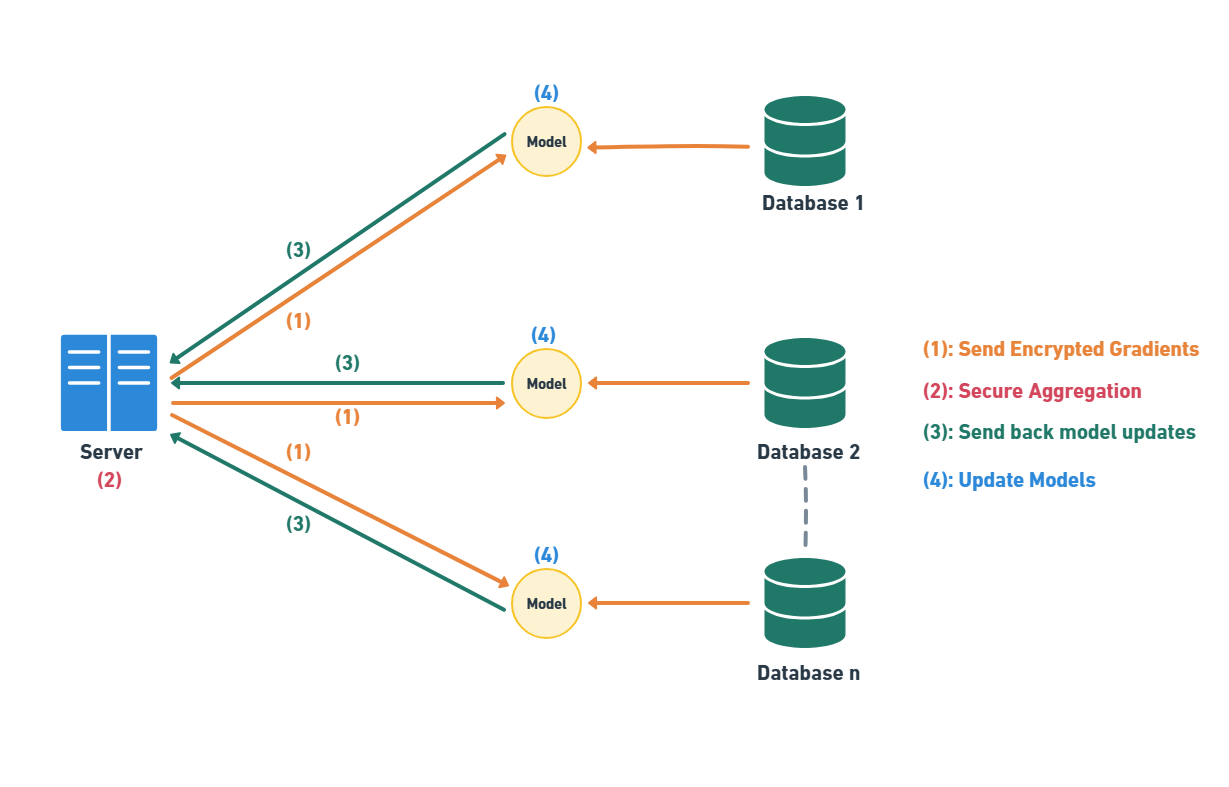
\includegraphics[width=0.75\linewidth]{Figures/diagram 1 (2).png}
    \caption{Horizontal Federated Learning}
    \label{fig:enter-label}
\end{figure}

Horizontal Federated Learning (HFL) is a decentralized machine learning approach in which multiple participants collaboratively train a shared global model without exchanging raw data. Each participant holds datasets with the same feature space, such as hospitals collecting identical health metrics, but with different data samples, ensuring both data privacy and compliance with protection regulations.

\textbf{Vertical Federated Learning (VFL)}
\begin{figure}[H]
    \centering
    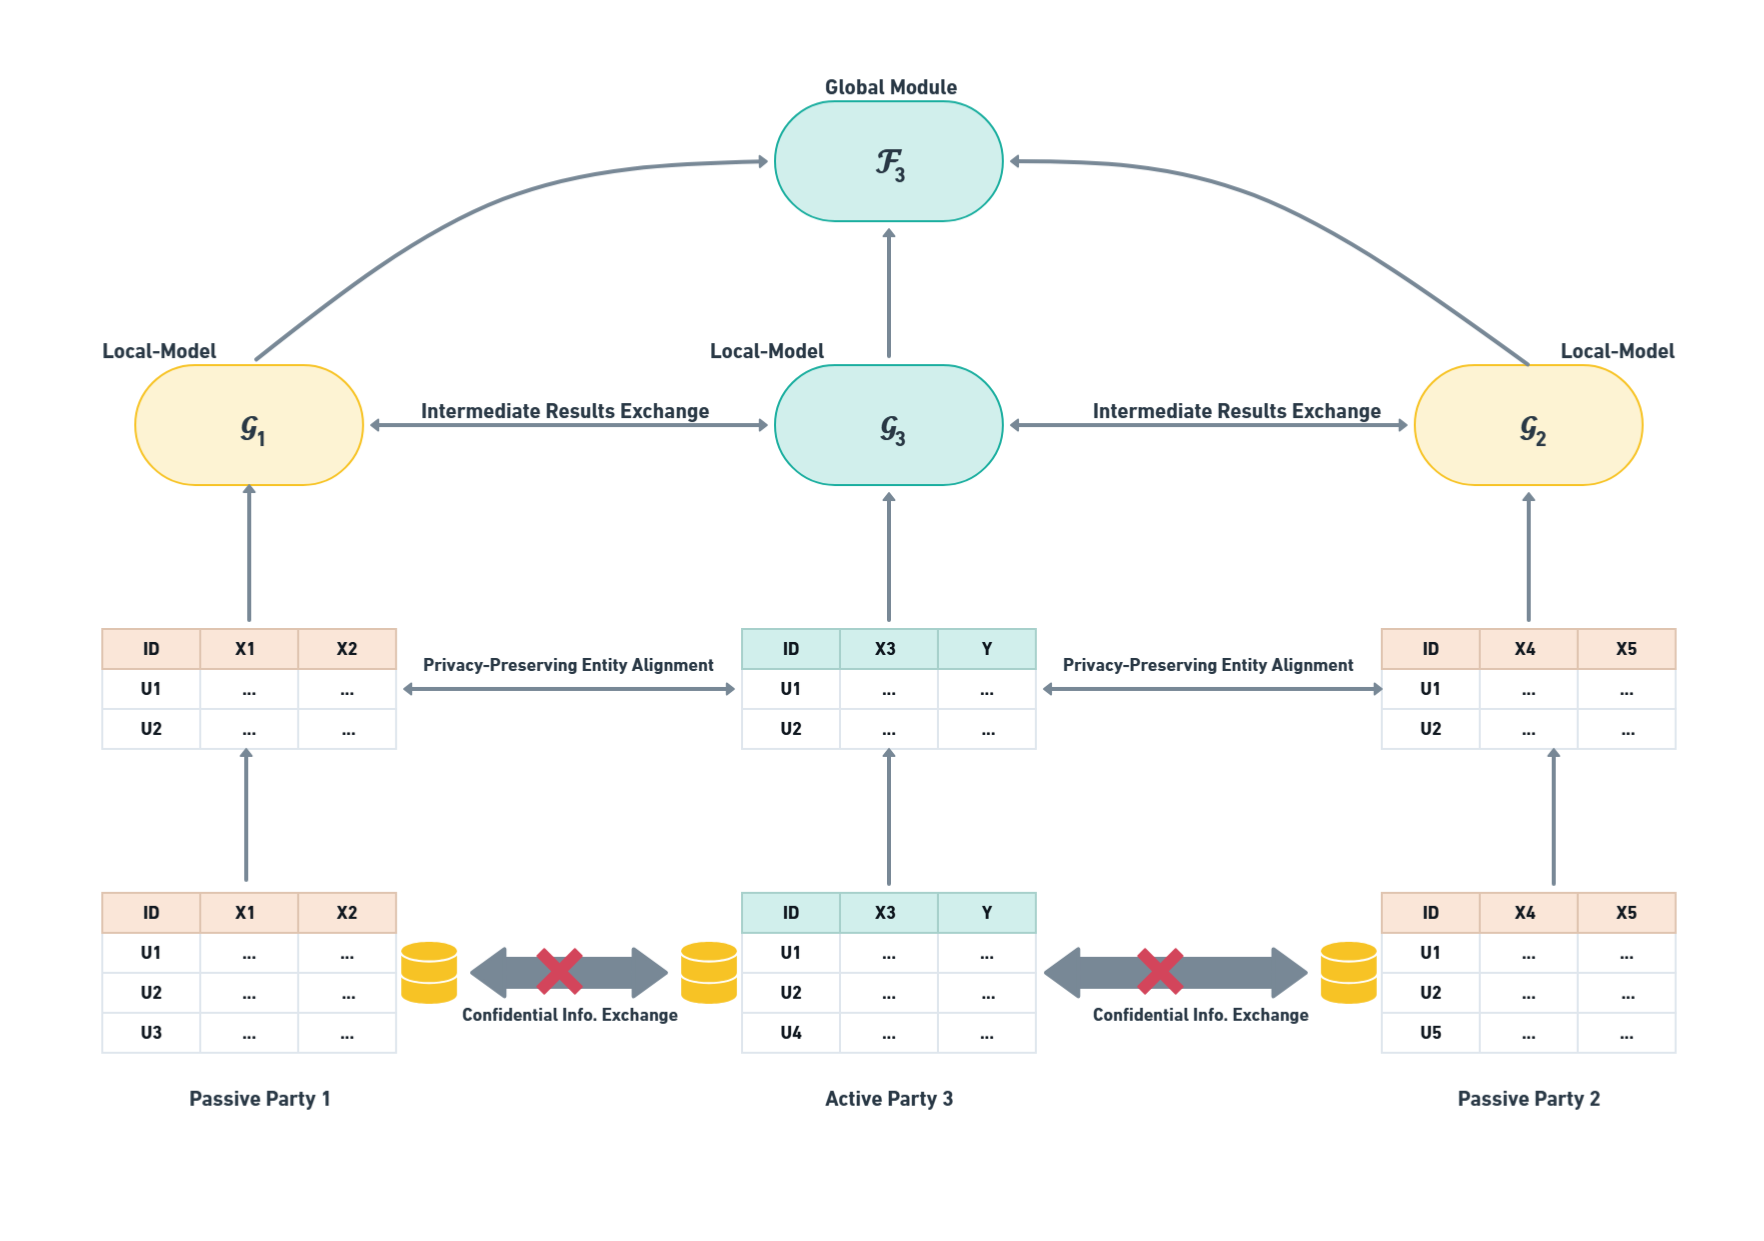
\includegraphics[width=0.75\linewidth]{Figures/VFL.png}
    \caption{Vertical Federated Learning}
    \label{fig:enter-label}
\end{figure}

Vertical Federated Learning (VFL) is tailored for scenarios where different organizations possess complementary features about the same individuals. For example, a bank can have access to a customer’s financial records, while a retailer holds their purchase history. By collaborating, these entities can train a more comprehensive model without revealing their raw data. In VFL, the feature space is partitioned, which means that each participant has a distinct subset of features for the same set of users,

\subsubsection{Based On Network Structure}

\begin{figure}[H]
    \centering
    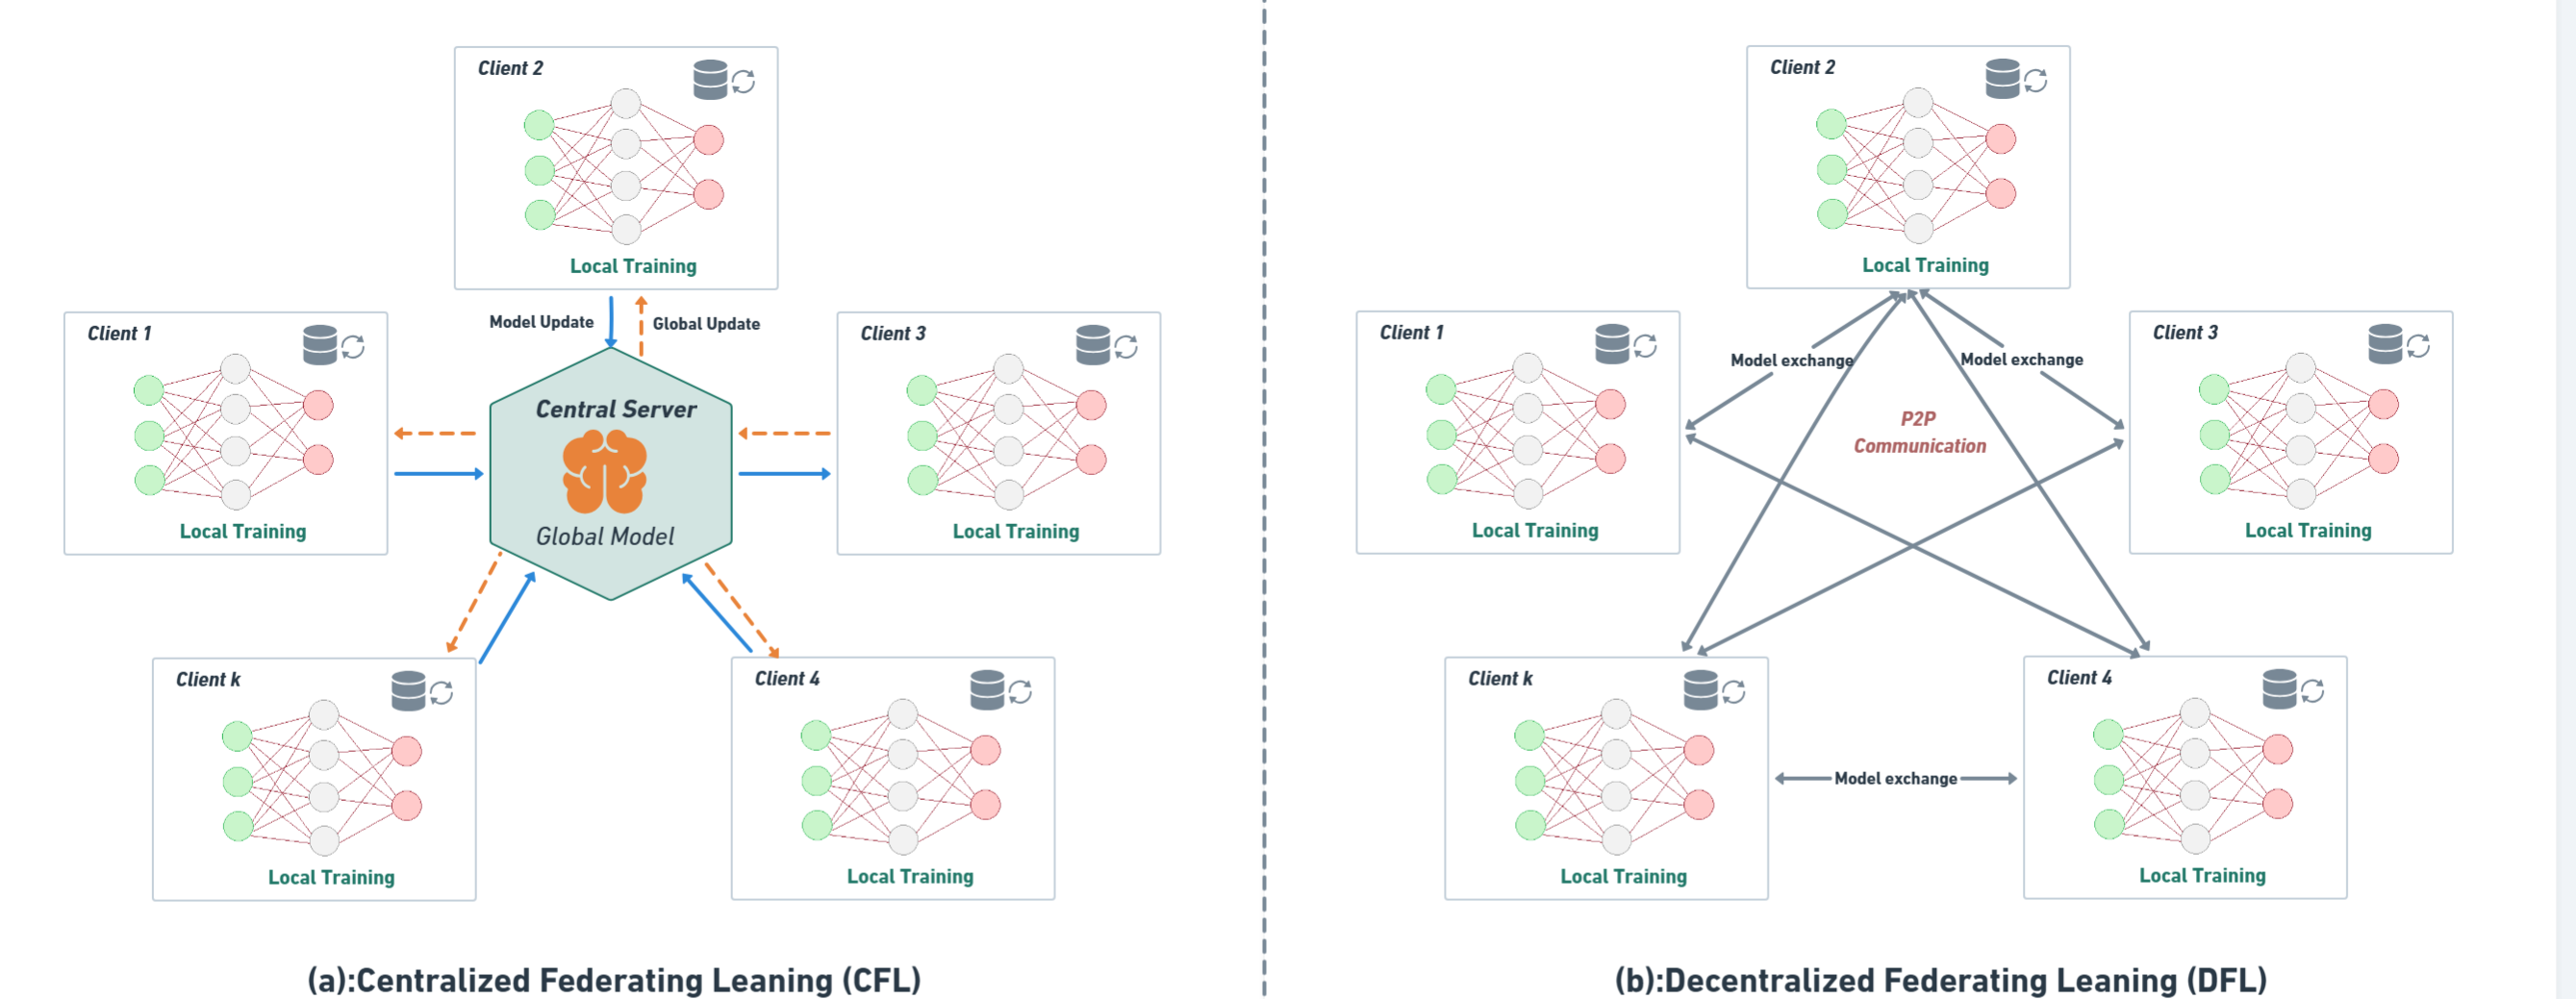
\includegraphics[width=1\linewidth]{Figures/network_based.png}
    \caption{Network Based Architecture}
    \label{fig:enter-label}
\end{figure}

Centralized Federated Learning (CFL) is a machine learning approach where a central server manages the coordination of training among multiple distributed clients. Each client trains a local model on its private data and periodically sends updates to the server. The server aggregates these updates to form a global model and redistributes it back to the clients. This setup allows data to remain local while still benefiting from collaborative learning across devices (Kairouz et al., 2021).

Decentralized Federated Learning (DFL) is a variation of federated learning that removes the need for a central server. Instead, clients communicate directly with each other in a peer-to-peer network to share model updates. Over time, these interactions lead to the development of a shared global model. DFL is particularly useful in environments where central coordination is not feasible or desired (Lalitha et al., 2019).

\subsection{Challenges and Solutions in Federated Learning}
\subsubsection{Privacy and Security Challenges}

Federated Learning (FL) faces significant challenges in maintaining data privacy and security during the collaborative training process. Since data remains on local devices, privacy-preserving techniques  such as encryption and differential privacy  are employed to prevent unauthorized access and ensure only aggregated model updates are shared [2].

Another major concern is the potential for malicious participants to inject biased or harmful updates into the training process. To mitigate this, secure aggregation protocols are implemented to verify the integrity and authenticity of model updates, ensuring the robustness of the final model.


\subsubsection{Communication and Resource Constraints}

Communication efficiency is crucial in FL, particularly when dealing with large-scale datasets or resource-constrained devices. To reduce communication overhead, techniques like model compression, quantization, and selective update transmission can be employed. These techniques reduce the amount of data transmitted between the local devices and the central server, which ultimately improves communication efficiency [2].


\subsubsection{Heterogeneity and Data Distribution}
Data and Model Heterogeneity Handling Strategies:
FL frameworks need to deal with heterogeneity in terms of data types, formats, and model architectures among various participating devices. Techniques such as transfer learning meta-learning, and model aggregation with model selection can be used to handle heterogeneity. These approaches permit the central server to adjust and combine models trained on different types of data or models with varying architectures [2].
Federated Transfer Learning and Meta-Learning Approaches:
Federated Transfer Learning facilitates the transfer of knowledge from a pre-trained global model to local models, which helps increase learning productivity and performance [2].



\section{System Design and Architecture}
\label{sec:system_design_and_architecture}

\subsection{General System Overview}
\label{ssec:general_system_overview}

The proposed Water Quality Monitoring System is a multilayered system that combines Internet of Things (IoT), Edge Computing, and Federated Learning (FL) technologies to provide a scalable and privacy-preserving solution for real-time water quality monitoring. As illustrated in Figure \ref{fig:system_architecture_high_level_overview}, the system has three main layers: the Edge Layer, the Intermediate Layer, and the Cloud Layer, each with respective roles that collectively facilitate intelligent data acquisition, localized processing, secure communication, and global model training.

\begin{figure}[H]
    \centering
    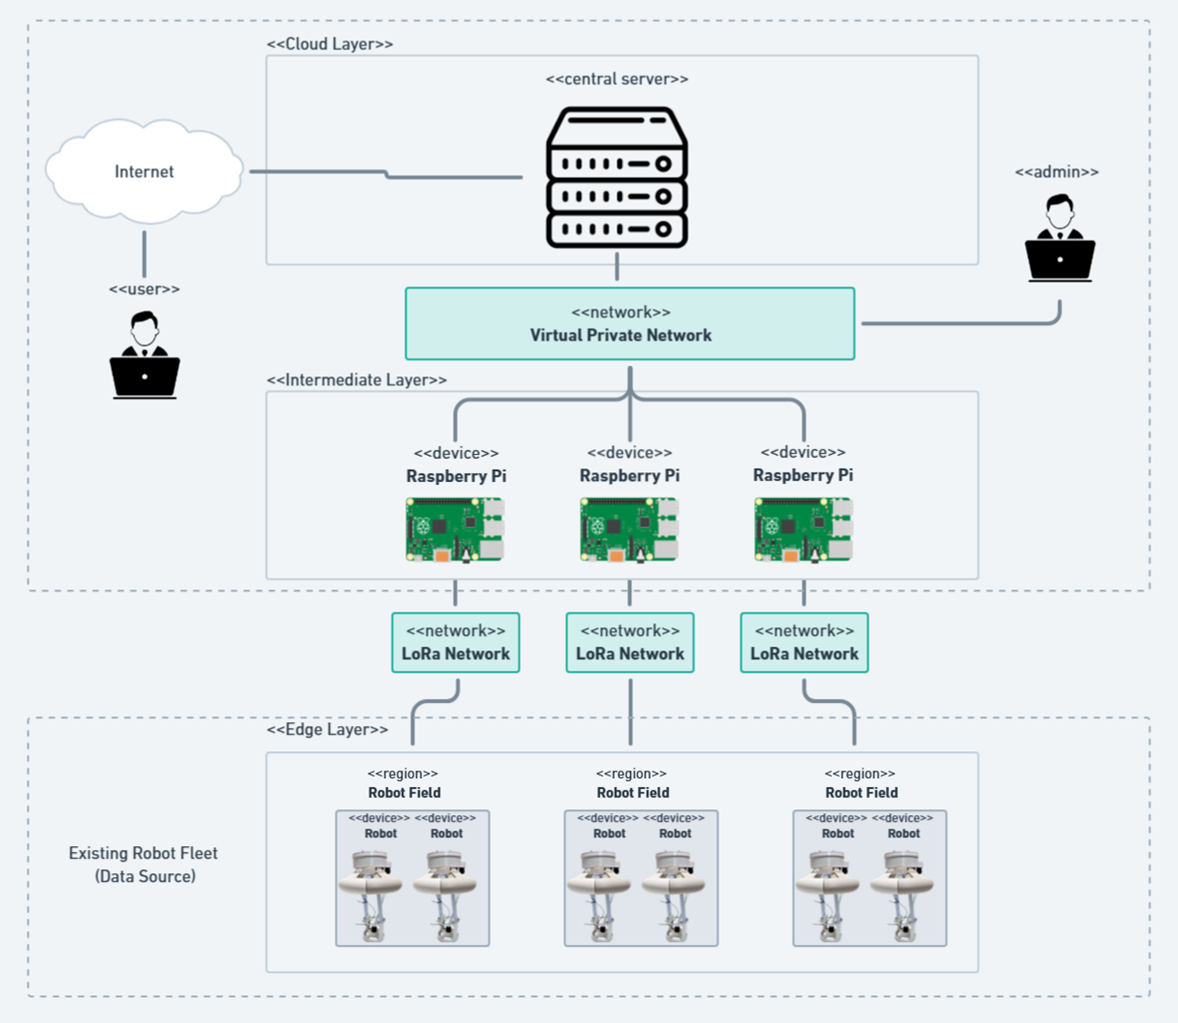
\includegraphics[width=0.75\linewidth]{Figures/system_architecture.png}
    \caption{General System Overview Diagram} % Updated Caption
    \label{fig:system_architecture_high_level_overview} % Updated Label
\end{figure}

The Edge Layer of the system consists of Water Quality Robots deployed in aquatic environments to enable distributed monitoring. The robots collect key water quality parameters and have low-power communication capabilities that allow them to transmit data wirelessly to the Intermediate Layer.

The Intermediate Layer, centered on Raspberry Pi units, functions as a bridge between sensor-equipped robots and the cloud infrastructure. It is responsible for aggregating data from multiple edge devices and performing a comprehensive preprocessing pipeline, including threshold-based filtering, basic machine learning-based anomaly detection, dynamic data cleaning. Furthermore, it initiates a federated learning process, training local machine learning models on the sanitized data and transmitting only encrypted model weight updates to the cloud.

Finally, the Cloud Layer serves as the central command and aggregation point. It comprises a Federated Learning server dedicated to orchestrating the global model aggregation process from updates received from various Intermediate Layer gateways. Alongside this, an Application Server manages overall system configurations, provides monitoring dashboards, and facilitates user interaction with the system.


\subsection{Detailed System Architecture and Component Breakdown} % Updated Subsection Title
\label{ssec:detailed_architecture_components}

The architecture depicted in Figure \ref{fig:global_architecture_detailed_components} illustrates a comprehensive and secure system designed for water quality monitoring, leveraging intelligent data processing through edge computing and federated learning. This diagram highlights the data flow and key interactions between components across the distinct system layers.

\begin{figure}[H]
    \centering
    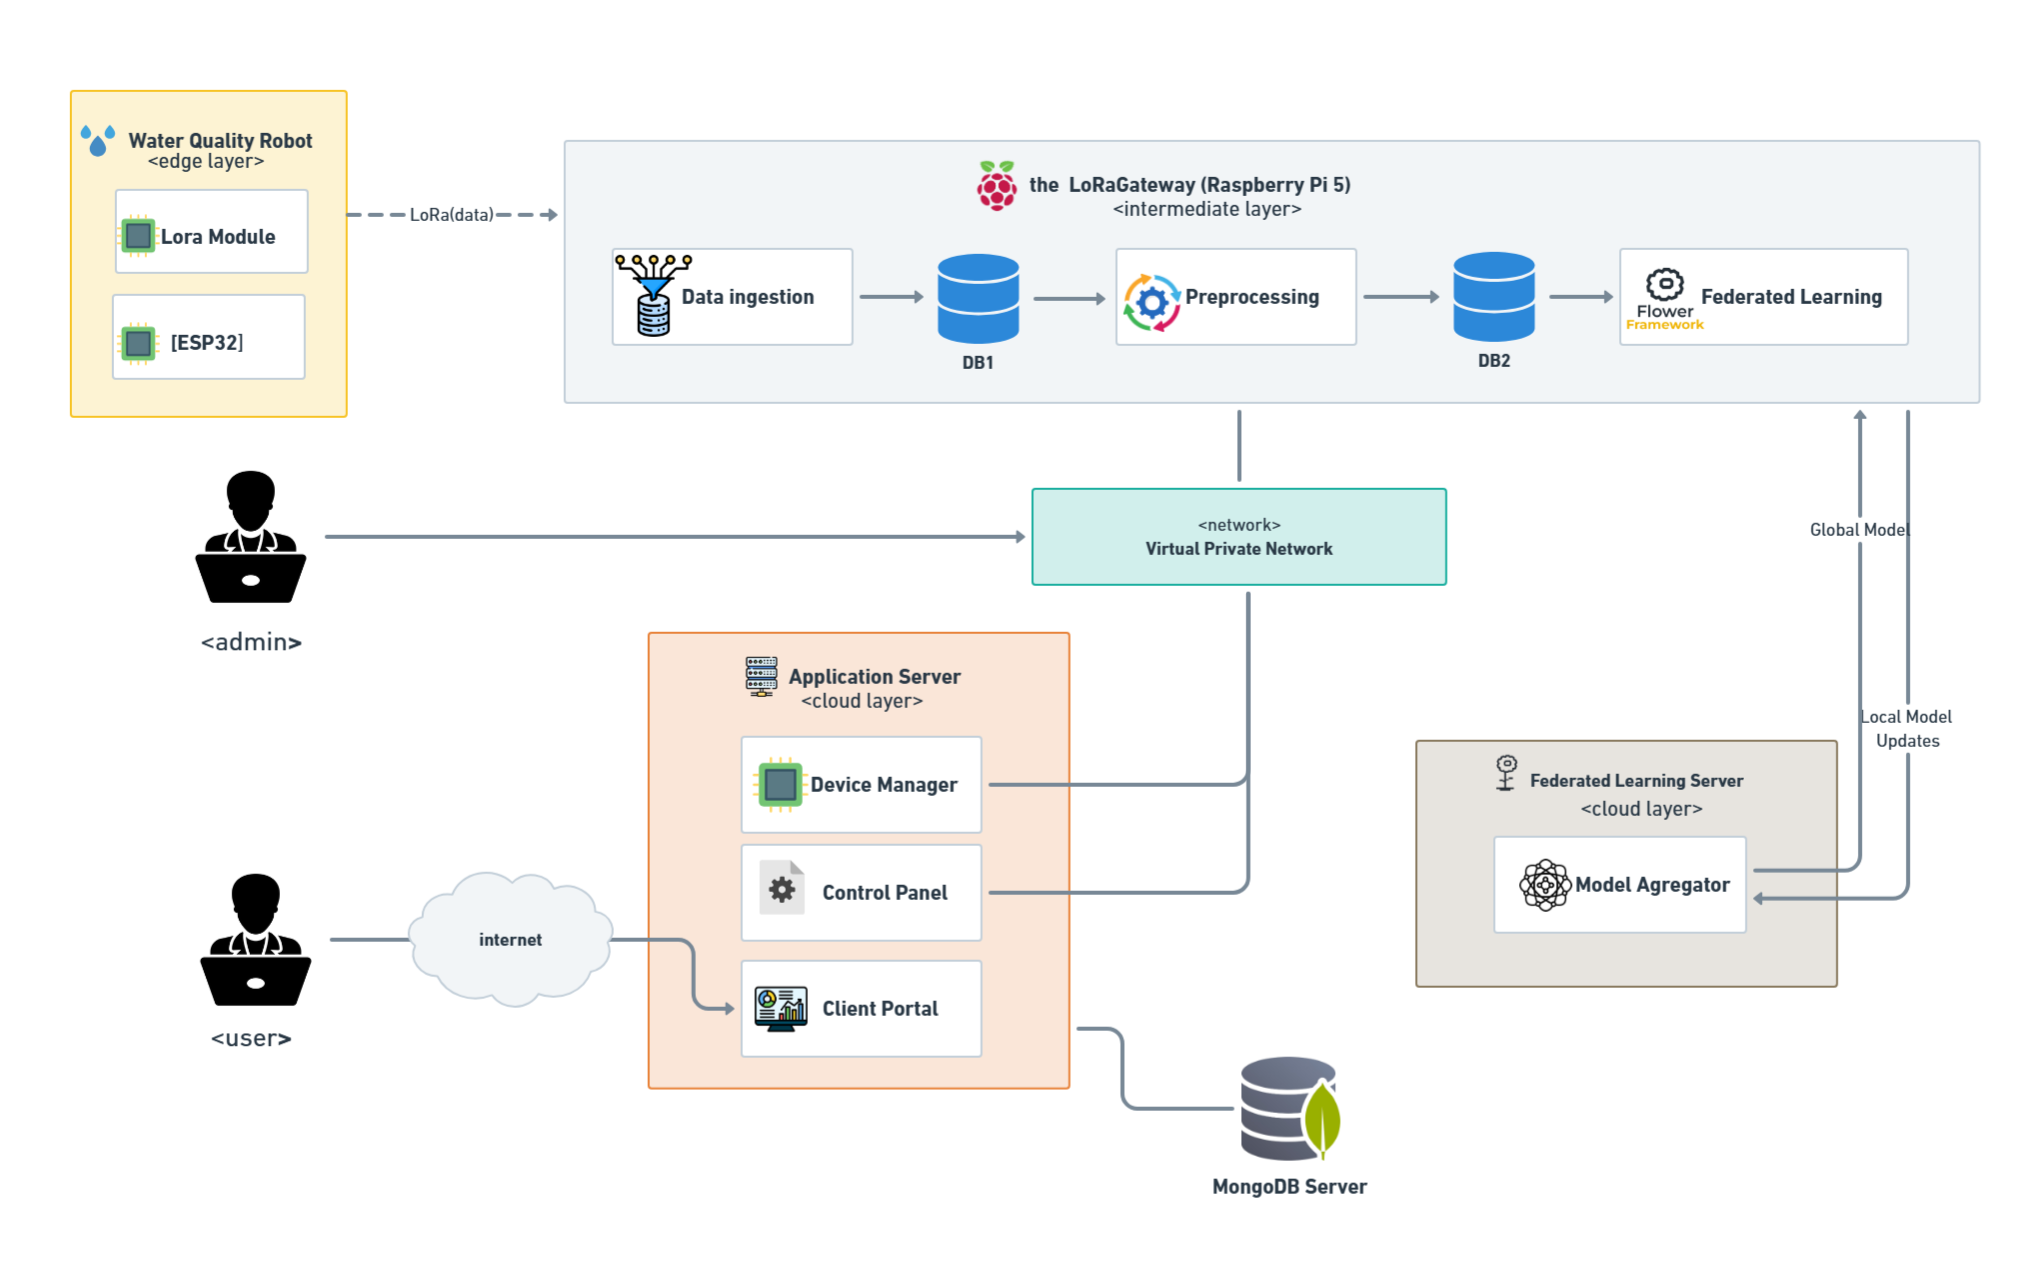
\includegraphics[width=0.75\linewidth]{Figures/GArchi1.png}
    \caption{Detailed Component Architecture Diagram}
    \label{fig:enter-label}
\end{figure}



Upon complete implementation, the edge layer will use Water Quality Robots as the primary data acquisition units. The design of these robots is based on the low-cost open-source smart buoy developed within the SmartWater project in Brussels, as detailed by Quevy et al. (2023). These autonomous robots will be equipped with a series of sensors to measure key water quality parameters, including pH, temperature, dissolved oxygen, conductivity, and potentially turbidity, consistent with the capabilities of the referenced buoy design. An ESP32 microcontroller will manage the onboard control and preliminary data processing, while a LoRa module will ensure long-range wireless communication. Sensor data, temporarily stored and formatted by the ESP32, will be transmitted via the LoRa protocol to a Raspberry Pi 5-based LoRa Gateway, a central component of the Intermediate layer.

Once the Raspberry Pi 5 in the intermediate layer receives raw data from these edge robots, it initiates a data processing pipeline. This begins with Data Ingestion, where incoming packets are decoded, transformed into a structured format, and stored temporarily in a local database (DB1). Following this, the Preprocessing phase applies filtering rules and machine learning models to detect anomalies and clean the data, with the resulting refined data stored in DB2, ready for training and analytics.

The core strength of this system lies in its integration of federated learning. The Raspberry Pi utilizes its private, preprocessed data from DB2 to train a local machine learning model using the Flower Federated Learning framework. Critically, only encrypted model updates are transmitted to the Federated Learning Server, which resides in the cloud layer and hosts a Model Aggregator. This server then aggregates updates from multiple participating gateways to build an improved global model, which is subsequently distributed back to the gateways. This iterative process enhances model accuracy while ensuring data privacy and decentralization.

The Raspberry Pi communicates with the Application Server in the cloud layer via APIs to receive configuration parameters and exchange operational data. The administrator can access the Application Server via a secure VPN to interact with its key components. The Control Panel provides full administrative control over the machine learning pipeline, including hyperparameter tuning, selection of anomaly detection methods, and regulation of the federated learning server. It also offers detailed statistics on system performance, anomaly reports, warnings, and notifications. The Control Panel allows the administrator to monitor and manage the operational status of all connected devices. In contrast, regular users can access only the Visualization Module, which provides a read-only interface for viewing historical and predicted WQI data. All relevant metrics and logs are persistently stored in a MongoDB server within the cloud infrastructure.

\subsubsection{Edge Layer}
\label{sssec:edge_layer_detail} % Now a subsubsection
The Edge Layer is envisioned as the primary data acquisition front-end of the Water Quality Monitoring System, responsible for direct in-situ environmental measurements. In the target deployment, this layer would consist of autonomous Water Quality Robots. The design specifications for these robots are based on the open-source "Smart Buoy" detailed by Quevy et al. in "Open Sensing System for Long Term, Low Cost Water Quality Monitoring" [*********** Reference Number for the Paper**************], selected for its proven capabilities in environmental sensing and LoRa communication.

These conceptual Water Quality Robots would incorporate an ESP32 microcontroller, a standard suite of sensors for parameters such as pH, temperature, dissolved oxygen (DO), electric conductivity (EC), and turbidity, and an RFM95W LoRa module for data transmission, mirroring the hardware architecture of the referenced Smart Buoy.

For the current phase of this research and system development, the data input from the Edge Layer is simulated using historical water quality datasets , built around an ESP32 and an RFM9x LoRa module, is utilized to send formatted data packets representative of what an actual Water Quality Robot would generate. This approach allows for the development and testing of the Intermediate Layer gateway, the Cloud Layer functionalities, and the federated learning mechanisms without requiring immediate deployment of the full physical robot fleet.

The function of this Edge Layer is therefore to provide periodic water quality data, which is then transmitted via LoRa to an Intermediate Layer gateway. This allows the project to focus on the data processing, communication protocols, and the federated learning architecture using realistic data inputs.
%TODO:
\subsubsection{Intermediate Layer}
\label{sssec:intermediate_layer_detail} % Now a subsubsection
The Intermediate Layer serves as a crucial local processing and learning hub, built around a gateway. This gateway is responsible for data ingestion, collecting raw sensor data from distributed Edge Layer robots.

\textbf{Gateway Hardware}

The gateway's hardware is centered around a \textbf{Raspberry Pi 5 with 8GB of RAM}, providing ample processing power for local data tasks and machine learning model training. For communication with the edge devices, it is equipped with an \textbf{Adafruit RFM95W LoRa Radio Transceiver Breakout}. This module facilitates the reception of data transmissions directly from the edge layer robots operating on the LoRa protocol. For local data storage, including raw sensor readings and processed datasets, the gateway utilizes a \textbf{64GB Class 10 microSD card}. The entire gateway assembly is powered by a 5V 5A power supply unit.


\textbf{Outlier Detection}

Collected data is first analyzed for anomalies. Using rule-based checks or lightweight machine learning, the gateway identifies outliers to prevent corrupted inputs from impacting the learning process. Anomaly metadata is retained and reported to the Application Server for transparency and long-term system oversight. The Application Server allows remote tuning of thresholds, detection methods, and update frequencies to adapt to changing environmental conditions or operational needs.

\textbf{Data Cleaning and Imputation}

Before imputation, the gateway trains local cleaning models to estimate missing values based on historical patterns. These models are updated periodically, and their performance is monitored. Accuracy metrics are reported to the Application Server. Once trained, these models are used in real time to impute missing or flagged data, ensuring the quality and consistency of training data. The Device Manager enables centralized control over model types, training intervals, and fallback strategies.

\textbf{Federated Learning Model Development and Training}

\label{par:fl_model_dev_train} % Label for paragraph if needed
The development and training of the Water Quality Index (WQI) predictive model in the gateway follow a structured two-stage approach.
\begin{enumerate}
    \item \textbf{Centralized Model Optimization:}
    
        Prior to federated deployment, an initial phase of centralized machine learning experimentation is conducted. This phase utilizes historical water quality datasets to:
        \begin{itemize}
            \item Perform feature engineering to derive a rich set of potential predictors from the base sensor readings and temporal information.
            \item Conduct iterative feature reduction and selection, evaluating feature importance to identify an optimal, parsimonious feature set.
            \item Explore various Recurrent Neural Network (RNN) architectures to determine a robust model structure suitable for time-series WQI prediction.
        \end{itemize}
        The primary outcome of this centralized stage is the selection of the more promising model architectures and their corresponding optimized feature sets.
    \item \textbf{Federated Learning Implementation:}
    
        With a well-defined model architecture and feature set derived from the centralized optimization phase, the gateway then participates in the federated learning process. Using the locally preprocessed and cleaned data, the gateway trains this selected local model as part of the Flower federated learning framework (as depicted in Figure \ref{fig:global_architecture_detailed_components}). It engages in regular training rounds orchestrated by the Federated Learning Server, contributing only its model updates (weights and gradients) rather than raw data. Ensuring data privacy, minimizes network load, and enables the collaborative building of a global WQI prediction model through decentralized intelligence.
\end{enumerate}

\textbf{Model Exploitation}

After completing the federated learning training and receiving an updated global model, the gateway waits for a signal from the Application Server before utilizing the locally refined model to make predictions on new incoming data. This ensures that predictions are based on the most current model version, and the gateway processes data locally without immediate server interaction for this inference step. Predictions are then transmitted to the Application Server for visualization and potential alert generation.


\textbf{Operational Workflow}

% The operational workflow at this gateway begins with data ingestion. Raw sensor data, received via LoRa from the distributed robots, is stored locally in its raw form (DB1 in Figure \ref{fig:global_architecture_detailed_components}) before undergoing further processing. A key characteristic of this architecture is that this layer does not transmit raw data to the cloud. Instead, it processes the data locally, shares only notifications and statistics with the Application Server, and actively participates in federated learning. Critical aspects of this layer's processing pipeline, such as outlier detection strategies and the training of cleaning models, are dynamically configurable via the Application Server .
The operational workflow starts with data collection from Sensors and Data Acquisition. For model training, Historical Data undergoes Outlier Detection and Data Cleaning before being used in a Federated Learning cycle; this involves local model training and server-based aggregation to create an improved global model. Separately, for prediction, recent Last Data Samples are also cleaned and fed into The best saved model to Predicting future values, which are then reported to the Server.
\begin{figure}[H]
    \centering
    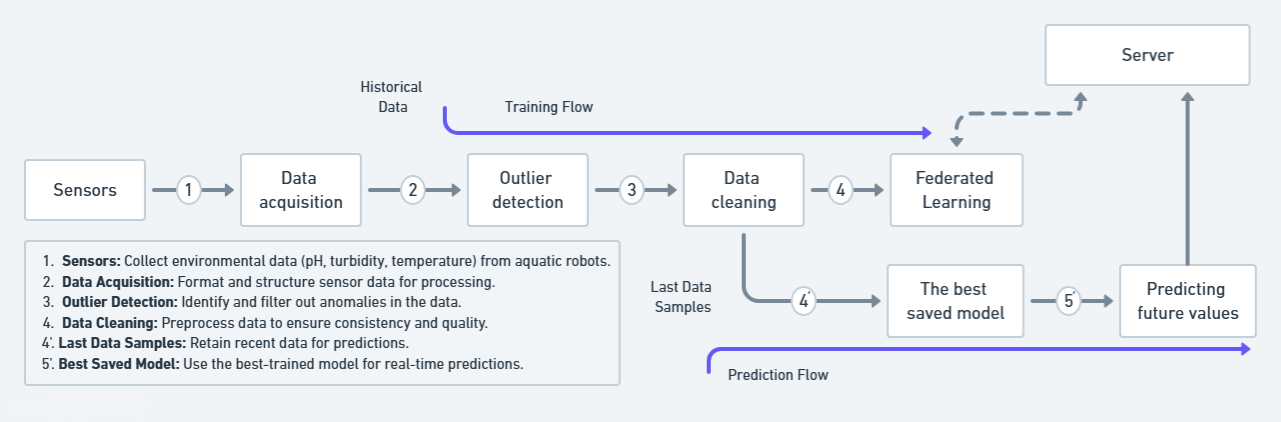
\includegraphics[width=1\linewidth]{Figures/Data Workflow.png}
    \caption{Data Processing Flow Diagram}
    \label{fig:enter-label}
\end{figure}

\subsubsection{Cloud Layer}
\label{sssec:cloud_layer_detail} % Now a subsubsection

\textbf{Federated Learning Server}

he Federated Learning Server coordinates the aggregation of locally trained model updates from gateways within the distributed system. Instead of centralizing data, each gateway trains a model on its local data and sends only weight updates to the server. These updates are combined using a federated averaging strategy to create a new global model, which is then redistributed to all gateways for the next training round. This iterative process enables continuous learning while preserving data privacy.

\textbf{Application Server}

The Application Server operates as a core software component hosted on the central AWS EC2 instance, alongside the Federated Learning Server and MongoDB. The cloud infrastructure, including these services, is secured using an OpenVPN server also running on the EC2 instance, establishing encrypted tunnels for communication with Intermediate Layer gateways.
It serves as the centralized control point for the overall Water Quality Monitoring System, bridging user interfaces with the gateways and the Federated Learning Server. As depicted in Figure \ref{fig:global_architecture_detailed_components}, it comprises several distinct modules:

\textbf{1. Client Portal }
The Client Application is a user-facing web platform that provides accessible water quality information and monitoring features to the public. It offers interactive tools such as regional water quality maps, real-time sensor data, and historical trends. Users can explore key features like environmental parameters and predictive analytics, and register to receive timely alerts on water quality changes in selected regions. The application focuses on delivering clear, actionable insights through an intuitive interface, supporting informed decision-making and community engagement.

\textbf{2. System Management Console (Control Panel):}
This Component provides secure administrator authentication and centralized control over system configurations and device management. Authorized administrators can onboard devices, adjust region-specific parameters  including anomaly detection thresholds and data cleaning models  and manage the scheduling of federated learning tasks such as model training and prediction. The module also delivers real-time monitoring and visualization of system notifications, anomaly occurrences, model performance metrics, and active alerts. All configuration and monitoring capabilities are accessible exclusively through a secured administrative interface.

\textbf{3. Device Management (Device Manager):}

% This component is central to managing interactions with the intermediate clients. It serves as the primary coordination point for dispatching operational commands to these distributed nodes, such as initiating federated model training cycles or triggering water quality prediction routines. To ensure these distributed tasks are performed reliably and at appropriate intervals. Furthermore, it is responsible for delivering client-specific configurations necessary for their operation and for processing the various outputs received from the devices, notably including operational alerts and crucial environmental data like water quality predictions.
This component directly manages and interacts with intermediate layer clients, primarily by delivering client-specific configurations to enable their designated tasks. It then serves as the central hub for dispatching operational commands like initiating model training or prediction routines based on system schedules, utilizing an internal scheduling mechanism for reliable execution. The Device Manager also processes outputs from these clients, handling operational alerts and ingesting their water quality predictions.

\newpage

\section*{Conclusion}
This chapter comprehensively outlined the methodological framework for the proposed Water Quality Monitoring System using Federated Learning. It detailed a robust multilayered architecture (edge, intermediate, cloud layers) with distinct, interconnected roles, from distributed data acquisition by autonomous robots to global model aggregation and system management. The critical functions of the intermediate LoRa gateway, encompassing data ingestion, preprocessing, local database management, and local model training, were elucidated, highlighting its role as a crucial hub for localized intelligence. Similarly, the responsibilities of the cloud layer, with its dedicated Federated Learning server for model aggregation and an Application Server for system configuration, monitoring, and user interaction, were thoroughly described. Furthermore, the chapter presented the data processing workflow, illustrating the systematic progression from raw sensor readings through cleaning and imputation to their effective utilization in the federated learning process for generating and refining predictive models. The strategic adoption of Federated Learning was central to this methodology, enabling a system that inherently ensures data privacy by keeping raw data localized, promotes scalability by distributing computational load, and enhances efficiency by minimizing communication overhead.

\pagebreak